\appendix
\newpage
\chapter*{\raggedleft\label{appendix1}ПРИЛОЖЕНИЕ}
\phantomsection\addcontentsline{toc}{chapter}{ПРИЛОЖЕНИЕ}
%\section*{\centering\label{code:appendix}Текст программы}



\begin{center}
\label{code:appendix}Текст программы
\end{center}



\begin{code}
\captionof*{listing}{\centering\label{code:brgame}Основной скрипт инициализации карты и алгоритма игры}
\vspace{-1cm}\inputminted[mathescape,linenos,frame=lines,fontsize=\tiny,breaklines]{csharp}{src/GameBoard.cs}
\end{code}

\begin{code}
\captionof*{listing}{\centering\label{code:click}Скрипт создания клеток по клику мыши}
\vspace{-1cm}\inputminted[mathescape,linenos,frame=lines,fontsize=\tiny,breaklines]{csharp}{src/TilemapClickHandler.cs}
\end{code}

\begin{code}
\captionof*{listing}{\centering\label{code:pi-example}Скрипт возвращения в главное меню}
\vspace{-1cm}\inputminted[mathescape,linenos,frame=lines,fontsize=\tiny,breaklines]{csharp}{src/BackMainMenu.cs}
\end{code}

\begin{code}
\captionof*{listing}{\centering\label{code:pi-example}Скрипт возвращения в главное меню}
\vspace{-1cm}\inputminted[mathescape,linenos,frame=lines,fontsize=\tiny,breaklines]{csharp}{src/BackMainMenu.cs}
\end{code}

\begin{code}
\captionof*{listing}{\centering\label{code:pi-example}Скрипт отрисовки границ карты}
\vspace{-1cm}\inputminted[mathescape,linenos,frame=lines,fontsize=\tiny,breaklines]{csharp}{src/BorderDraw.cs}
\end{code}

\begin{code}
\captionof*{listing}{\centering\label{code:pi-example}Скрипт динамической камеры}
\vspace{-1cm}\inputminted[mathescape,linenos,frame=lines,fontsize=\tiny,breaklines]{csharp}{src/CameraAdjuster.cs}
\end{code}

\begin{code}
\captionof*{listing}{\centering\label{code:pi-example}Скрипт перехода на сцену редактирования}
\vspace{-1cm}\inputminted[mathescape,linenos,frame=lines,fontsize=\tiny,breaklines]{csharp}{src/EditorButton.cs}
\end{code}

\begin{code}
\captionof*{listing}{\centering\label{code:strMap}Скрипт запуска созданной карты в режиме редактирования}
\vspace{-1cm}\inputminted[mathescape,linenos,frame=lines,fontsize=\tiny,breaklines]{csharp}{src/EditorStartMap.cs}
\end{code}

\begin{code}
\captionof*{listing}{\centering\label{code:pi-example}Скрипт выхода из игры}
\vspace{-1cm}\inputminted[mathescape,linenos,frame=lines,fontsize=\tiny,breaklines]{csharp}{src/ExitButton.cs}
\end{code}

\begin{code}
\captionof*{listing}{\centering\label{code:pi-example}Скрипт создания паттерна}
\vspace{-1cm}\inputminted[mathescape,linenos,frame=lines,fontsize=\tiny,breaklines]{csharp}{src/Pattern.cs}
\end{code}

\begin{code}
\captionof*{listing}{\centering\label{code:pi-example}Скрипт выключения заставки}
\vspace{-1cm}\inputminted[mathescape,linenos,frame=lines,fontsize=\tiny,breaklines]{csharp}{src/PressAnyKey.cs}
\end{code}

\begin{code}
\captionof*{listing}{\centering\label{code:pi-example}Скрипт выключения заставки по нажатию любой кнопки}
\vspace{-1cm}\inputminted[mathescape,linenos,frame=lines,fontsize=\tiny,breaklines]{csharp}{src/PressAnyKey.cs}
\end{code}

\begin{code}
\captionof*{listing}{\centering\label{code:rndB}Скрипт генерации и запуска карты в режиме Случайная Генерация}
\vspace{-1cm}\inputminted[mathescape,linenos,frame=lines,fontsize=\tiny,breaklines]{csharp}{src/RandomButton.cs}
\end{code}

\begin{code}
\captionof*{listing}{\centering\label{code:lvl}Скрипт готового паттерна в режиме Загрузить Карту}
\vspace{-1cm}\inputminted[mathescape,linenos,frame=lines,fontsize=\tiny,breaklines]{csharp}{src/LevelTransition.cs}
\end{code}

\begin{figure}[H]
	\centering
	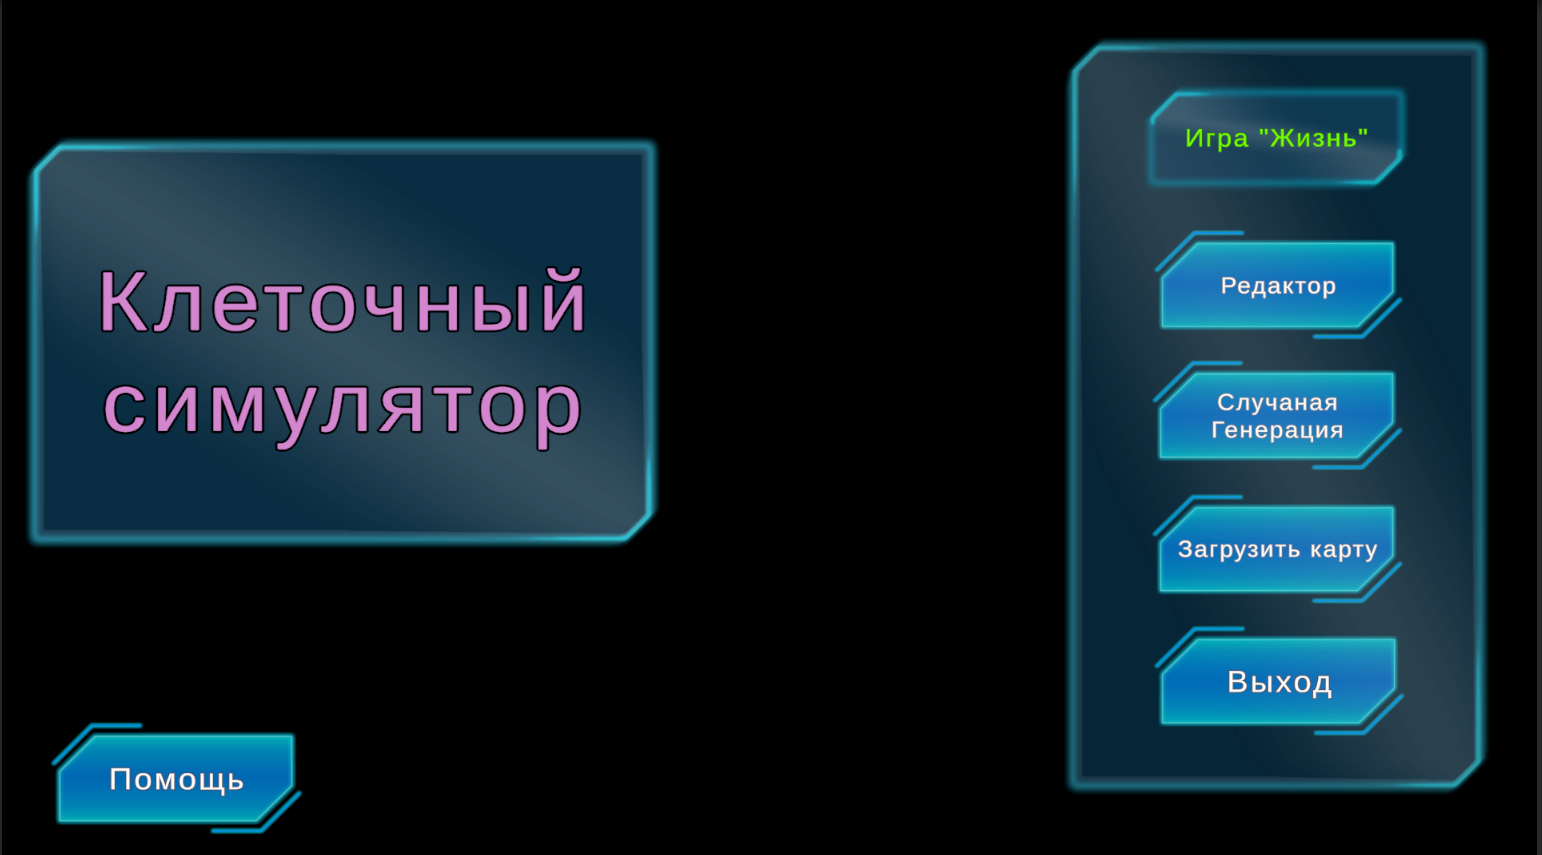
\includegraphics[width=1\textwidth]{images/MainMenu.png}  
	\caption{Главное меню <<Игры жизнь>>.}
	\label{MainM}
\end{figure}

\begin{figure}[H]
	\centering
	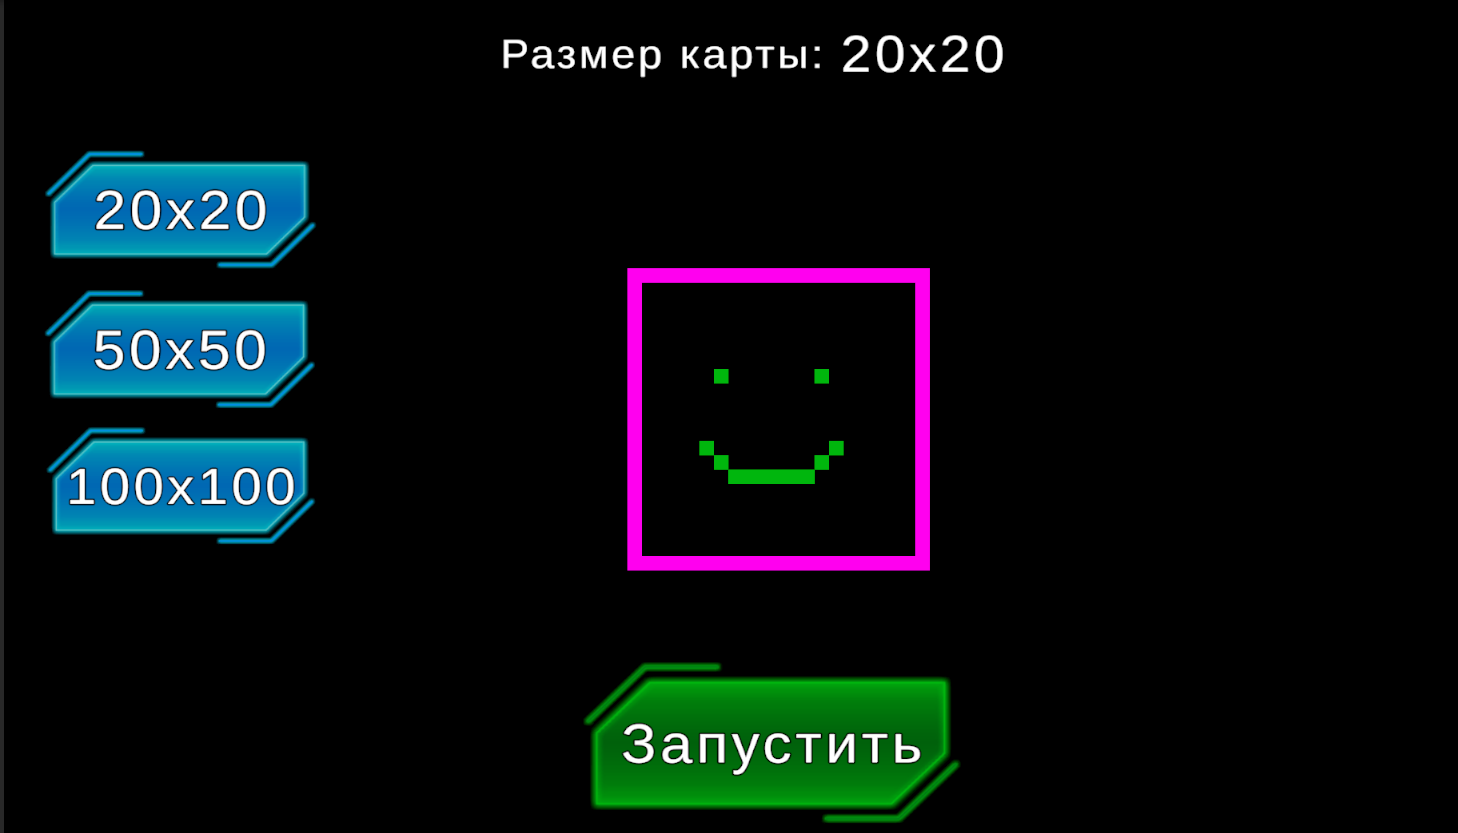
\includegraphics[width=1\textwidth]{images/Editor.png}  
	\caption{Редактор.}
	\label{Editor}
\end{figure}

\begin{figure}[H]
	\centering
	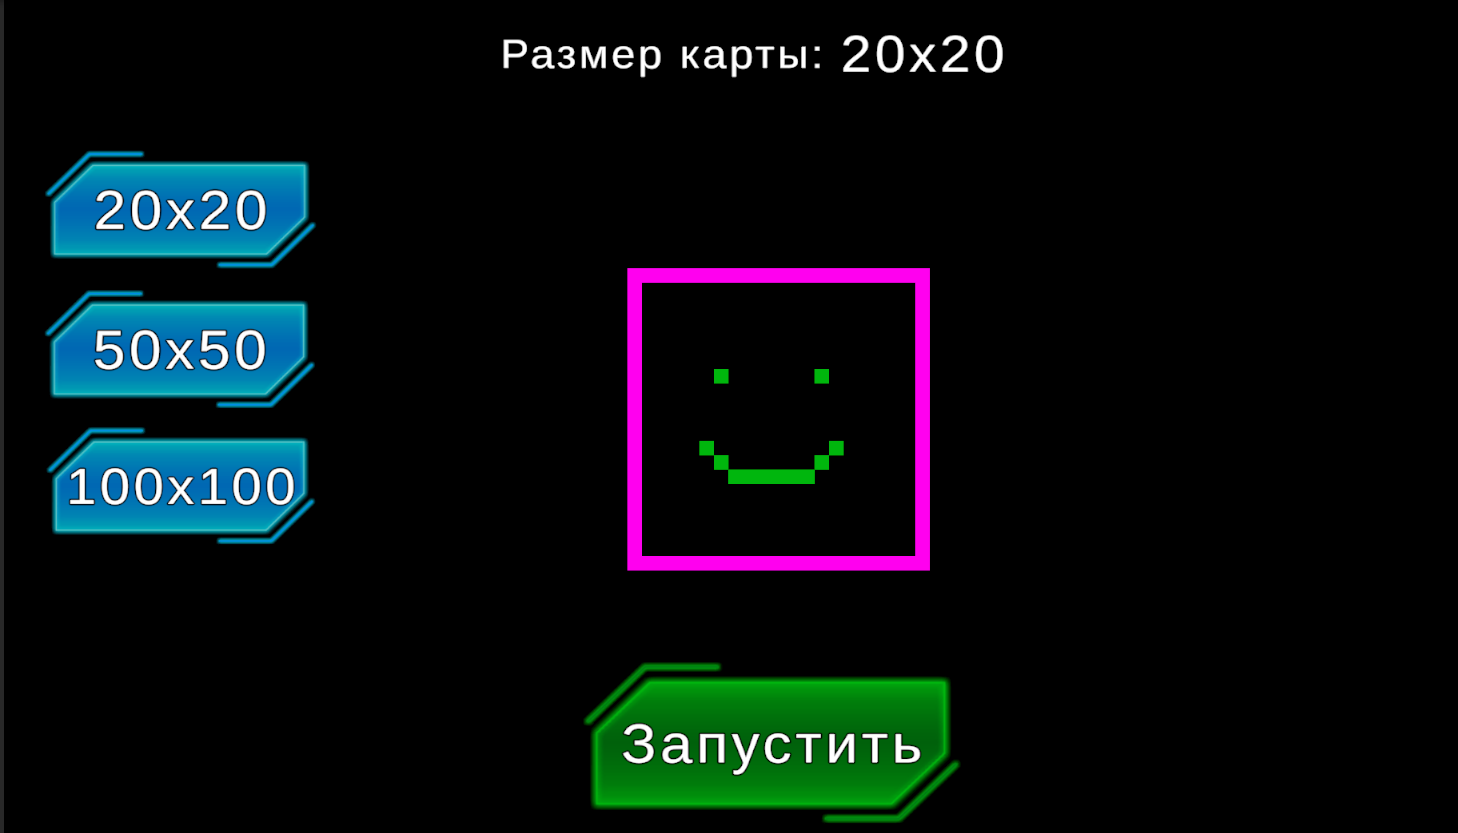
\includegraphics[width=1\textwidth]{images/Editor.png}  
	\caption{Окно редактора.}
	\label{Editor}
\end{figure}

\begin{figure}[H]
	\centering
	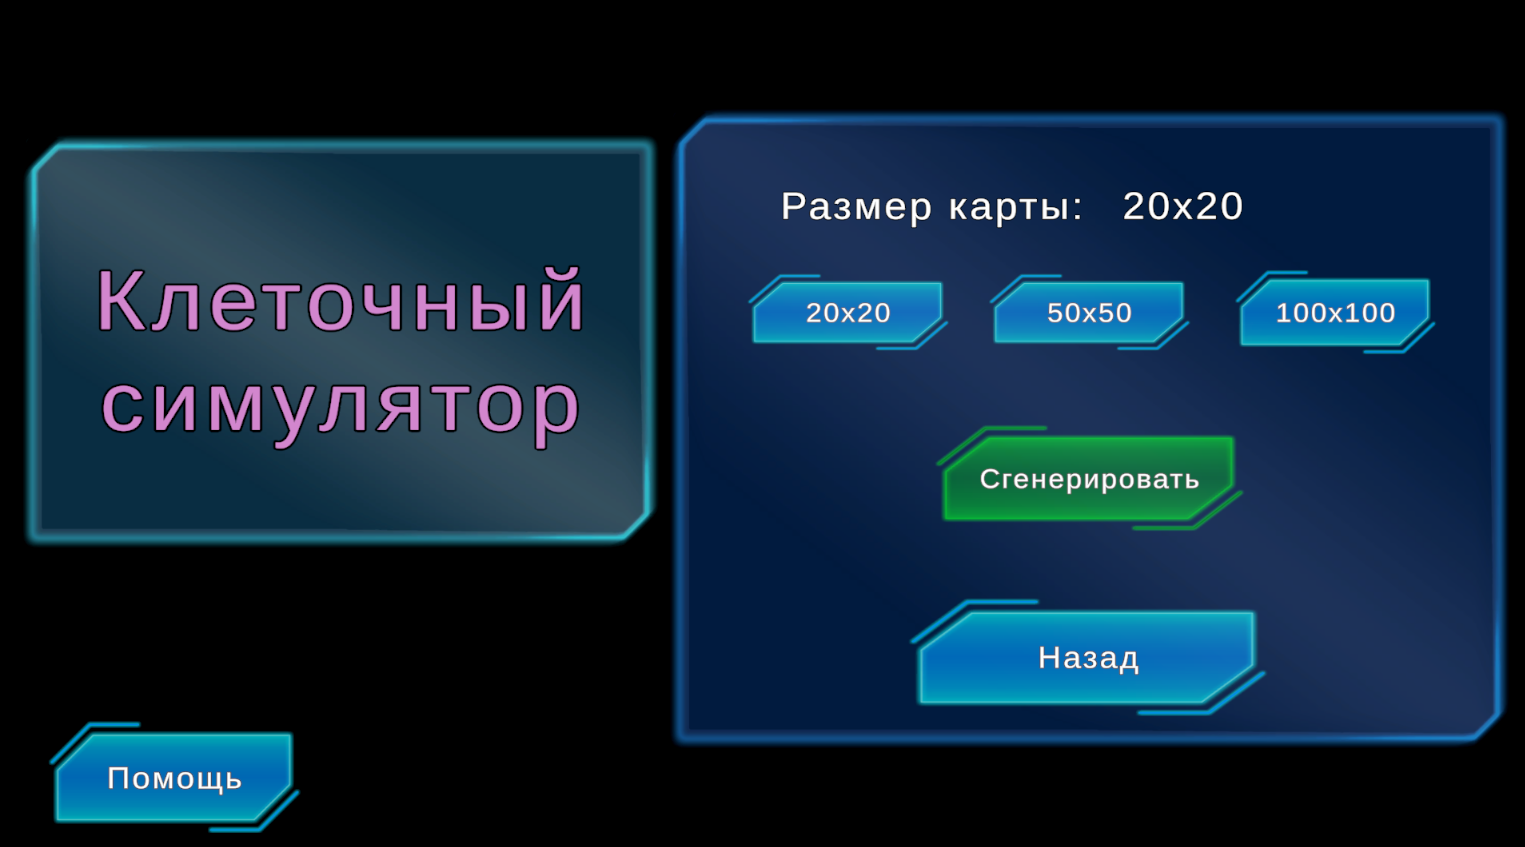
\includegraphics[width=1\textwidth]{images/rand1.png}  
	\caption{Панель Случайной генерации.}
	\label{rand}
\end{figure}

\begin{figure}[H]
	\centering
	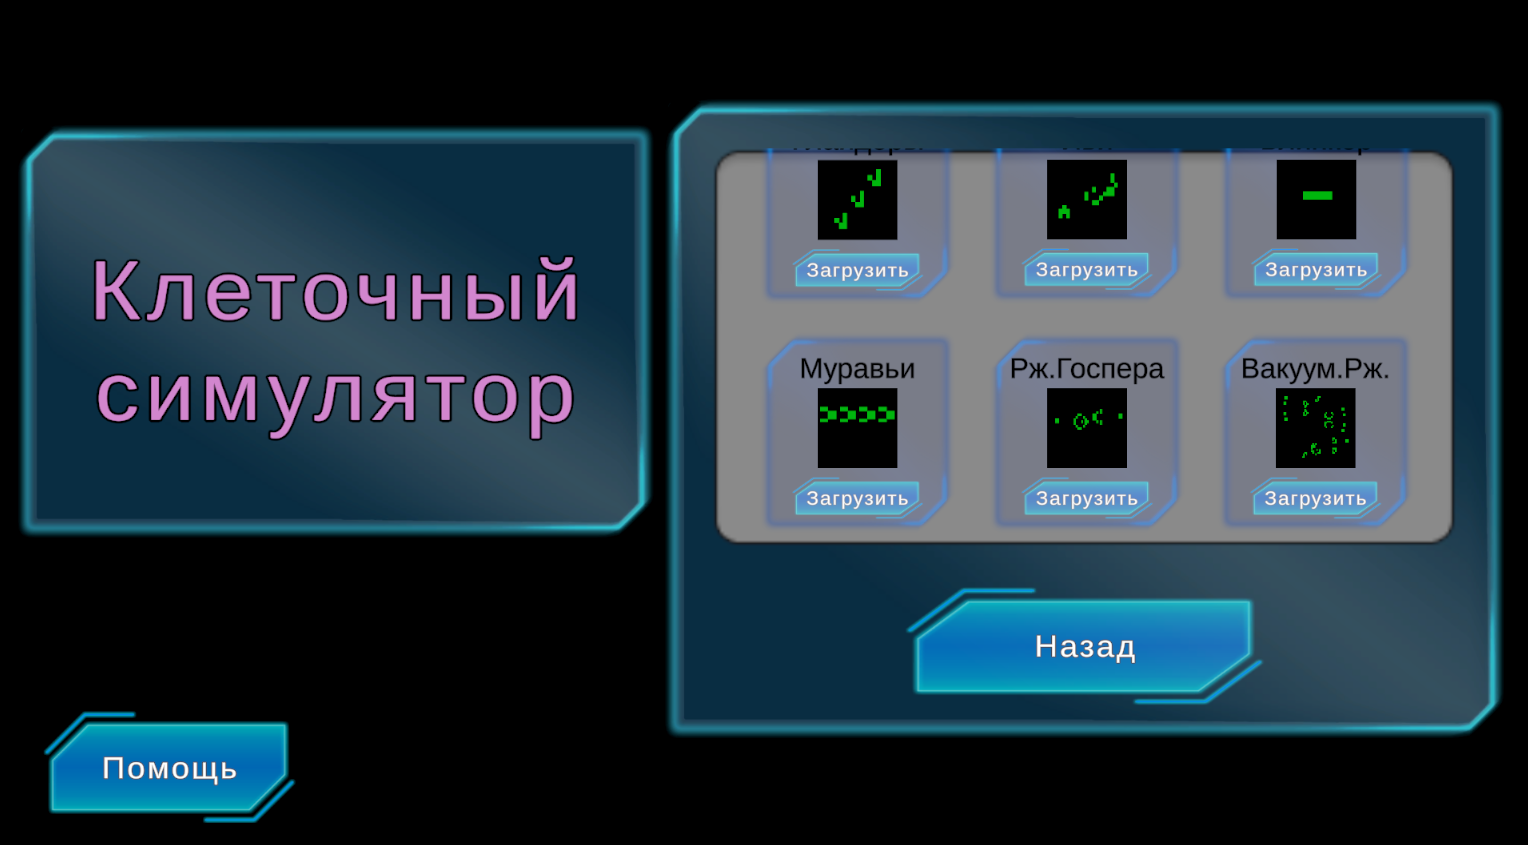
\includegraphics[width=1\textwidth]{images/downld.png}  
	\caption{Панель Загрузки карт.}
	\label{downl}
\end{figure}

\begin{figure}[H]
	\centering
	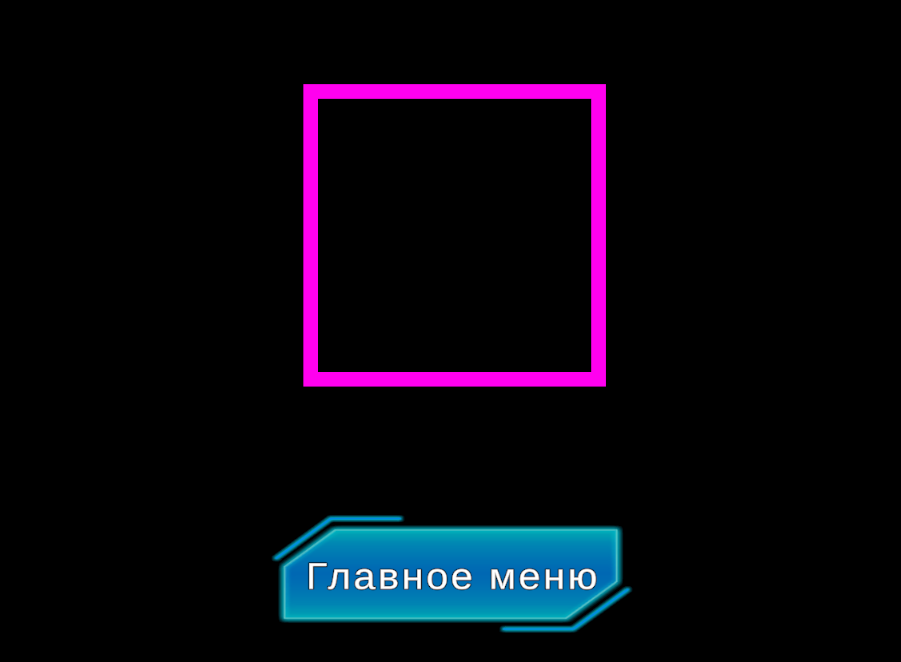
\includegraphics[width=1\textwidth]{images/map.png}  
	\caption{Игровое поле.}
	\label{map}
\end{figure}

\begin{figure}[H]
	\centering
	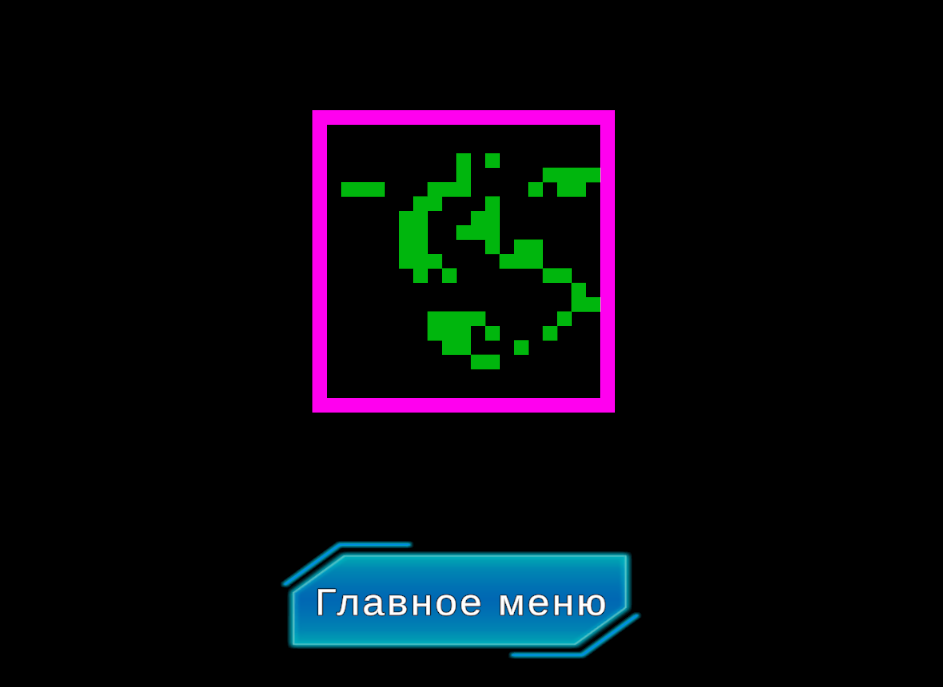
\includegraphics[width=1\textwidth]{csae-report-master/images/rand2.png}  
	\caption{Симуляция.}
	\label{uim}
\end{figure}